\scanpage{45}

En particulier, on trouve la deuxième classe de Chern d'une courbe \(C\) dans la surface \(Y\):
\[
C^2(\underline O_C)=\tfrac12[C^2-CK_Y+f_*(k_{\unsure{\widetilde C|C}})]
\]
où \(f:\widehat C\mathbin{\text{---}}Y\) est l'homomorphisme canonique dans \(Y\) de la normalisée \(\widetilde C\) de \(C\), et \(k_{\widetilde C}\) la classe canonique sur \(\widetilde C\). Si \(Y\) est compacte, et \(\widetilde C\) de genre \(g\), on trouve, en prenant les \(\unsure{K_2|\kappa_2}\) des deux mbs
\[
\unsure{K_2|\kappa_2}(C^2(\underline O_C))=\tfrac12[C^2-CK_Y+2g-2]=\tfrac12(C^2-CK_Y)+g-1
\]

\margin{PEWRITER}
\figure{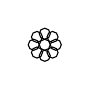
\begin{tikzpicture}[scale=.2]\draw (0,0) circle (.35);\foreach \a in {0,45,...,315}{\draw (\a:.7) circle (.35);}\end{tikzpicture}}
\margin{ARGENTINA LINEN \unsure{TYPEWRI}}
\margin{44}
